\section{Part 1}
\subsection{Part A}
		Using the circuit shown in figure \ref{fig:circuit1}, we measured the drain current with $V_{bs} = 0 V$, $V_{gs} = 2.5 V$, and $0V \le V_{ds} \le 5 V$.
		\FloatBarrier

		\begin{figure}[h!]
		\centering
		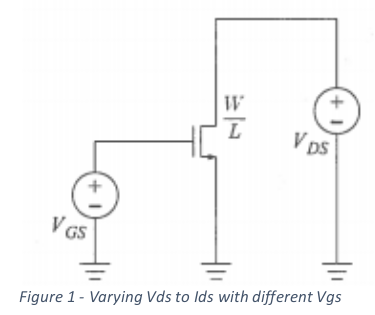
\includegraphics[scale=0.75]{../images/circuit1.png}
		\caption{The circuit tested in part 1.}
		\label{fig:circuit1}
		\end{figure}

		\FloatBarrier
		From the data we collected for $I_{ds}$ and $V_{ds}$, we were able to find that the NMOS entered triode mode at $V_{ov} \approx 0.1 V$. 
		As soon as the drain voltage surpassed $V_{ds}=0.1 V$ we saw a dramatic increase in drain current.
		This increase began to taper off around $V_{ds}\approx0.8V$, as the NMOS entered saturation mode. 
		We can approximate the threshold voltage to be $V_{tn} = 1.7 V$.

		\begin{equation}
		\label{eq:threshold}
		V_{tn} = V_{gs} - V_{ds} = 2.5 V - 0.8 V = 1.7 V
		\end{equation}

		\FloatBarrier

		\begin{figure}[h!]
		\centering
		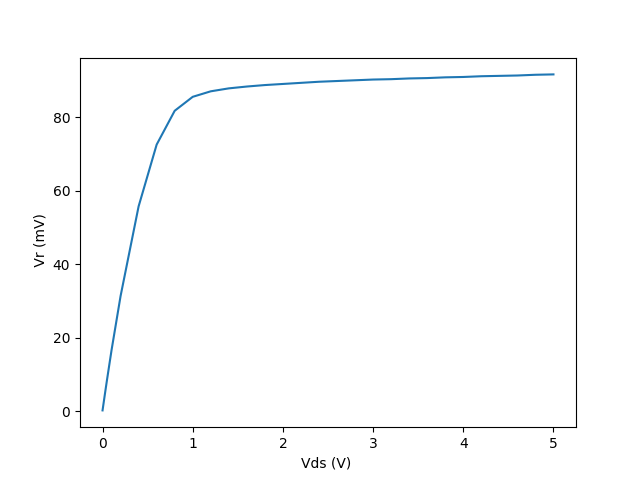
\includegraphics[scale=0.75]{../data/nmos.png}
		\caption{The resulting $I_{ds}$ vs $V_{ds}$ graph for $V_{gs}=2.5V$.}
		\label{fig:nmos}
		\end{figure}

		\FloatBarrier
		During testing we noticed capacitive effects when moving from triode down to cutoff. 
		If we were increasing drain voltage from below the point of cutoff to move into triode mode the drain voltage of $V_{ds}=0.15V$ resulted in $I_{ds}\approx 166 \mu A$;
		however, when moving from saturation or triode mode down into cutoff mode a drain voltage of $V_{ds}=0.15 V$ produced $I_{ds}\approx 310 \mu A$.
		We believe this is due to the capacitive effects of the MOSFET structure.

		\subsection{Part B}
		During Part B we used the same parameters from Part A, except the gate voltage was increased to $V_{gs} = 5V$. 
		We can see from the $I_{ds}$ and $V_{ds}$ curve in figure \ref{fig:nmos_5v} the NMOS is operating in triode mode over the range of $0.8 \le V_{ds} \le 3.2V$.

		\FloatBarrier

		\begin{figure}[h!]
		\centering
		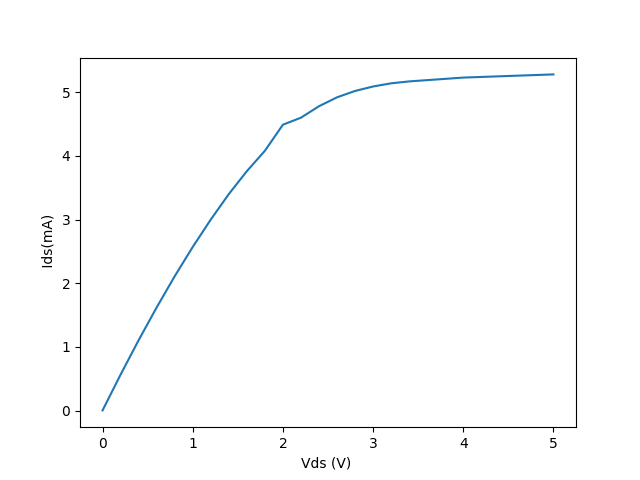
\includegraphics[scale=0.75]{../data/nmos_5v.png}
		\caption{The resulting $I_{ds}$ vs $V_{ds}$ graph for $V_{gs}=5V$.}
		\label{fig:nmos_5v}
		\end{figure}

		\FloatBarrier
		We can check our approximation from part A for the threshold voltage of $V_{tn} = 1.7 V$.
		
\begin{equation}
	\label{eq:thresh_5V}
		V_{ds} = V_{gs} - V_{tn} = 5 V - 1.7 V = 3.3 V.	
\end{equation}
This result for $V_{ds} = 3.3 V$ as the edge of saturation agrees well with the measured data. 
We can see on the curve the drain current stays fairly constant after approximately $V_{ds}=3.2 V$.
After comparing the percentage of change in the drain current and drain voltage, we find that after $V_{ds} = 3.2 V$ the change in the drain current stays at less than one percent, despite the change in drain voltage of about five percent. 
This result proves that our result of $V_{tn} = 1.7 V$ is a good approximation for the threshold voltage.
